\documentclass[../tesis.text]{subfiles}

\chapter{Marco teórico}
	\section{Robots de servicio}
		%Conceptos


		%Estado del arte
		Dado que este trabajo se centrará en los robots de servicio, en partícular en una metodología de detección y manipulación de objetos, resulta fundamental poner en evidencia el panorama actual de los robots de servicio. La idea general de la robótica de servicio doméstico ha existido desde hace mucho tiempo, pero es un tema de investigación relativamente joven. El objetivo de crear robots de servicios útiles y autónomos que puedan interactuar con seres humanos y objetos en el mundo real en un entorno natural plantea un gran número de problemas sin resolver en muchas disciplinas científicas.\\
		%\vspace{0.2in}

		Recientemente, el progreso en estos campos de investigación, así como el progreso y la normalización en el desarrollo de hardware y software, ha llevado a un aumento en la disponibilidad de recursos, métodos y componentes para el desarrollo  de Robots de servicio doméstico . Por ello estamos cada vez más cerca de convivir con robots de servicios de manera exitosa en diversos lugares, por ejemplo hospitales \cite{hospitalRobots}, oficinas, construcciones, o tiendas departamentales \cite{robotsInStores}.\\
		%\vspace{0.2in}


		Estos desarrollos han sido posibles gracias a herramientas de código abierto como lo es Ubuntu, ya que ha servido como base para el desarrollo de software especializado para robots, por ejemplo ROS \cite{rosEpage}. Este conjunto de librerías especializadas para robots pueden llegar a ser muy patículares y estar enfocados a una sola área de invetigación de las antes mencionadas, por ejemplo: Carmen \cite{carnegieMellon}, un conjuto de liberías y algoritmos de control para navegación de robots, desarrollados por la universidad Carnegie Mellon\cite{cMellonEpage}.\\
		%\vspace{0.2in}

		En la parte de simulación se cuenta con ejemplos como el USARSim \cite{balakirsky2006}, rviz \cite{rVizEpage} o Gazebo \cite{gazeboEpage}. Por lo que respecta a los algoritmos de visión computacional existen bibliotecas de código abierto por ejemplo OpenCV \cite{openCV} el cual tiene un gran campo de aplicaciones\cite{bradski2000}. Por lo que corresponde a los kits standar de hardware, podemos mencionar la construcción de robots de plataforma standar por ejemplo VolksBot \cite{wisspeintner2007} y las plataformas bases por ejemplo ActivRobots \cite{ActivRobots}, Pepper \cite{pepperEpage}, Asimo \cite{asimoEpage} ha hecho posible desarrollar software de manera más rápida y eficiente.\\
		%\vspace{0.2in}

		\begin{figure}[htb]
			\begin{center}
			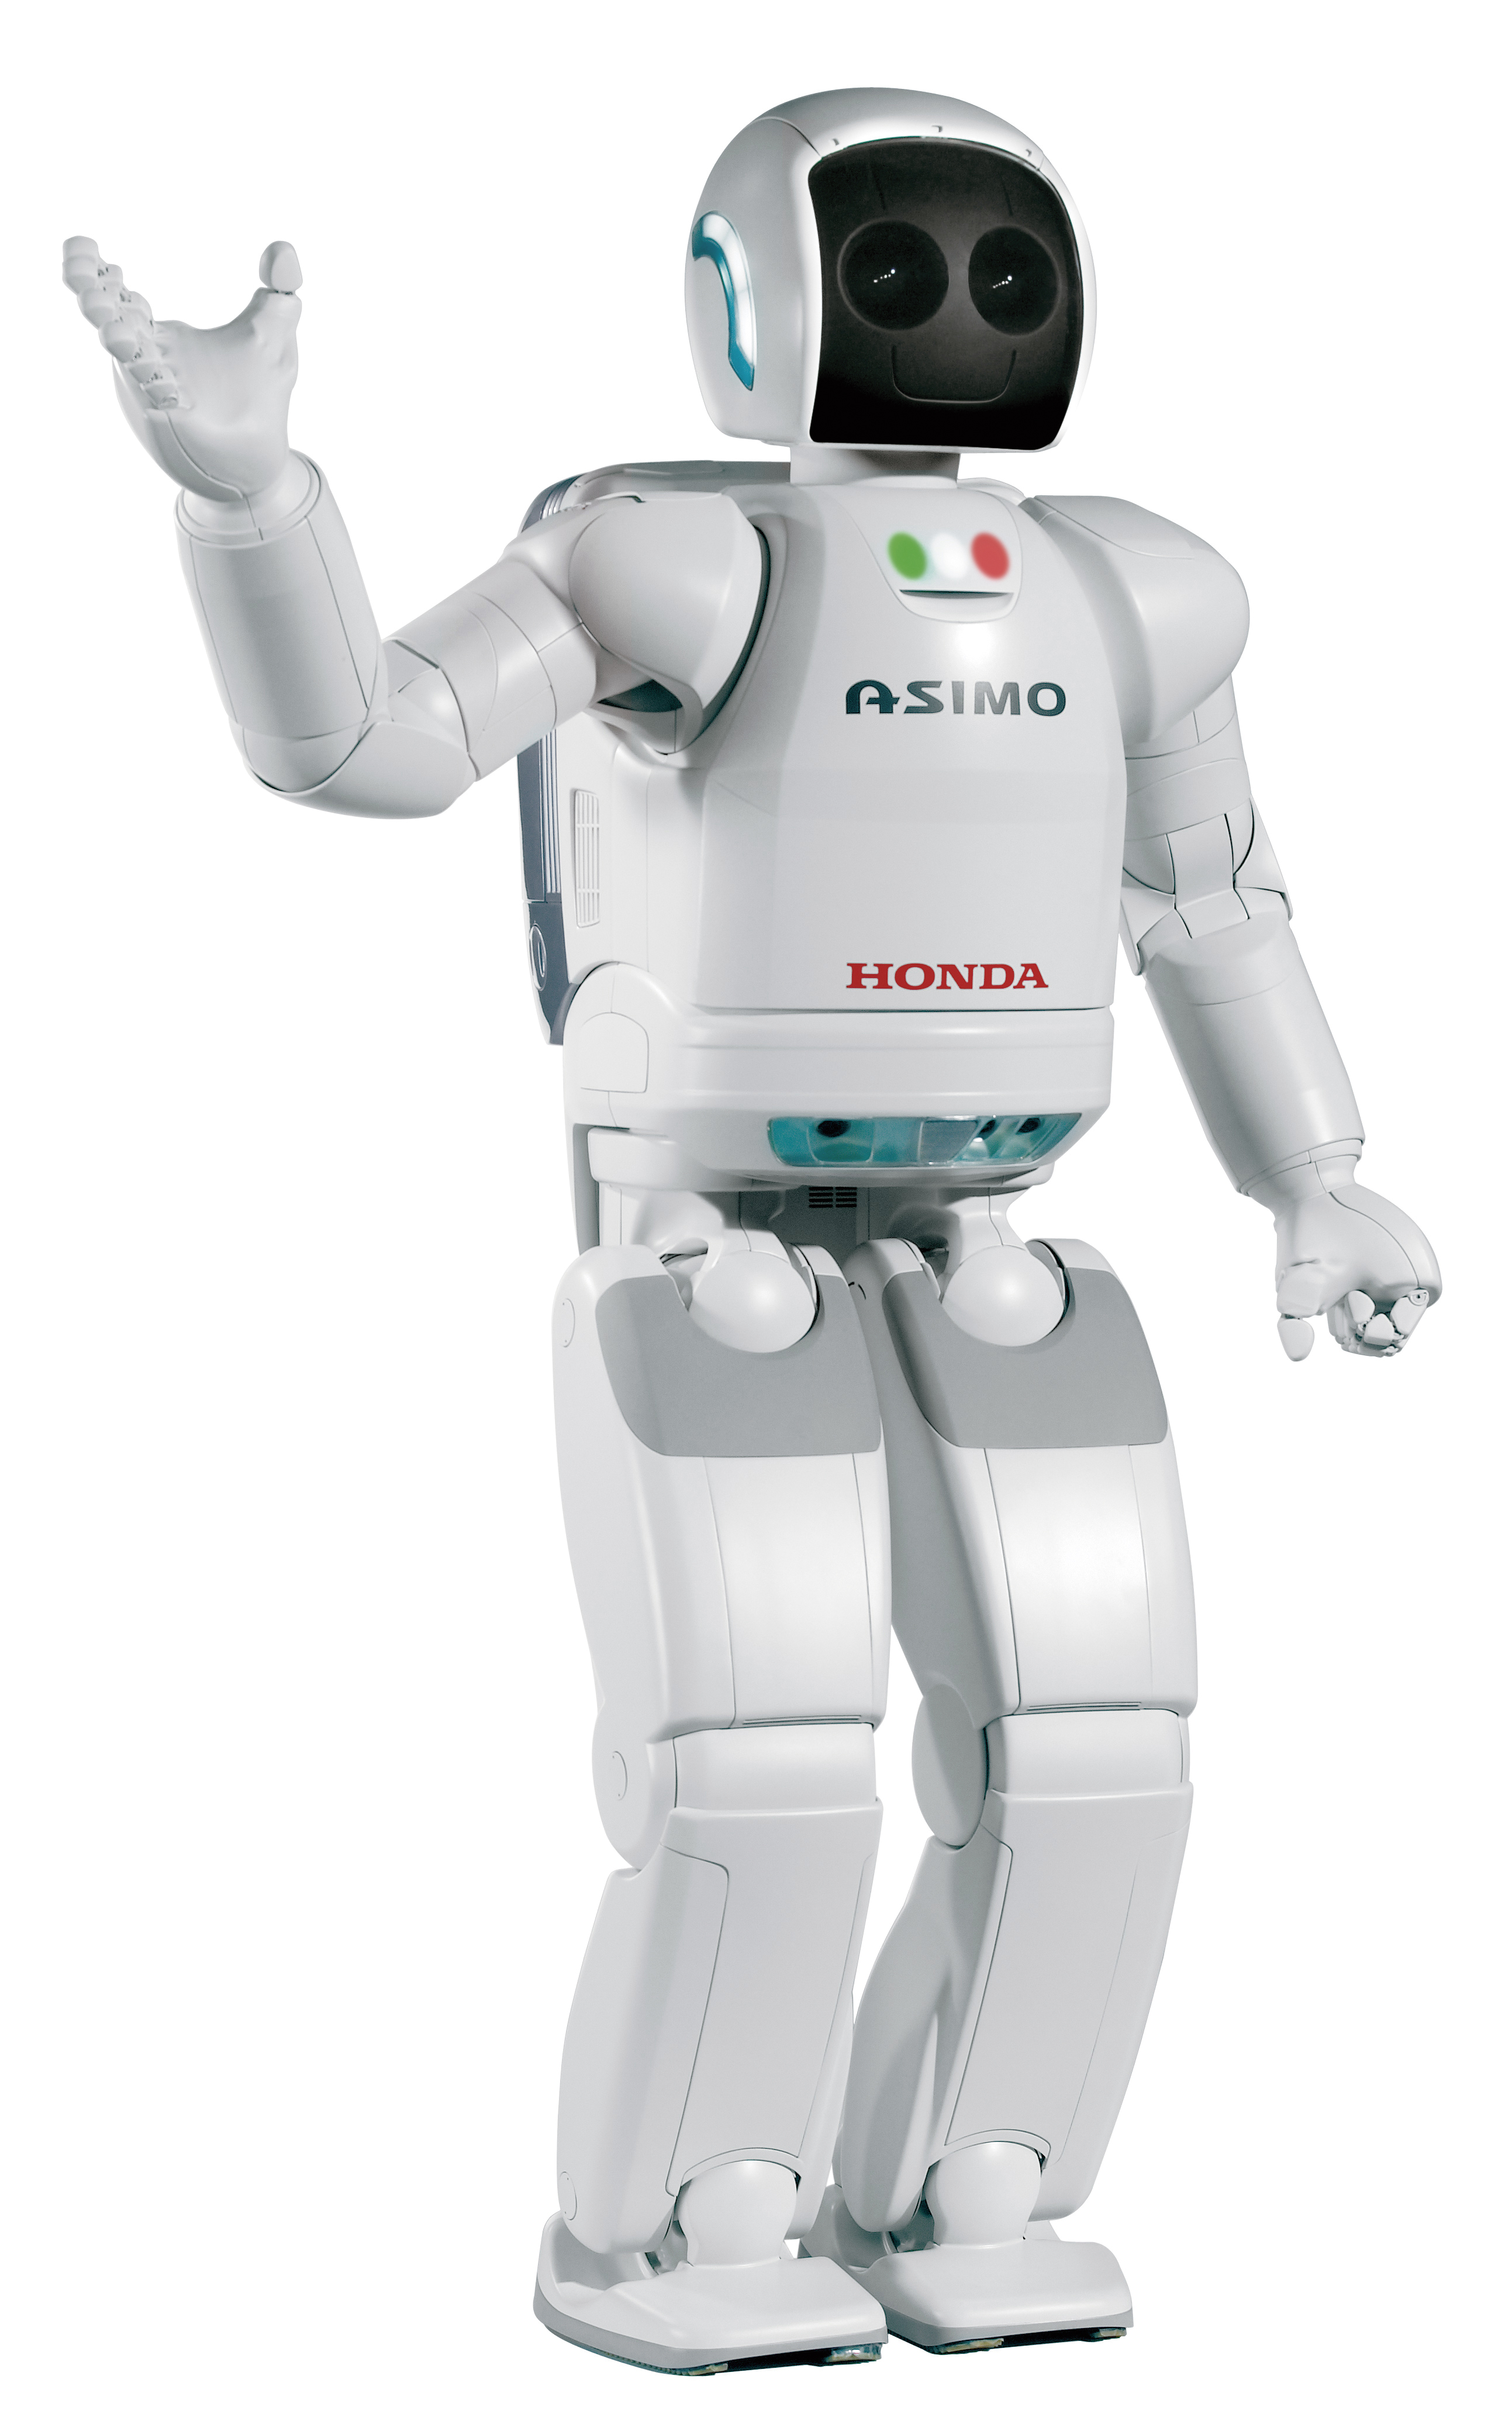
\includegraphics[width=3.5cm, height=5cm]{/asimo.jpg}
			\end{center}
		\end{figure}



%%% Fundamentos de Manipuladores
%%  ---------------------------------

	\section{Fundamentos básicos de Robots Manipuladores}
		La manipulación adecuada de objetos es una característica imprescindible en los robots de servicio dadas las condiciones de su entorno y las tareas cotidianas que le podemos asignar a dicho robot. Una posible solución a la problemática de la manipulación de objetos es la incorporación de manipuladores seriales a una base móvil; sin embargo se debe tener encuenta que los objetos a ser manipulados se encuentran en condiciones aleatorias de posición y orientación, estas características implican que el manipulador serial debería ser capaz de alcanzar una posición (x, y, z) con cualquier orientación (roll, pitch, yaw).\\

		Los robots manipuladores clásicos presentan una configuración antropomórfica serial, que hace semejanza con un brazo humano. La arquitectura típica de un manipulador consiste en una serie de barras rígidas unidas entre sí mediante el uso de acticulaciones rotacionales o prismáticas. De manera general cada articulación logra su movimiento gracias a un actuador y a la adición de algunos elelmentos complementarios como sensores de posición y de velocidad\cite{baturone2005}.\\

		*Los robots manipuladores clásicos están caracterizados, desde el punto de vista mecánico, por una serie de propiedades talez como los grados de libertad, el espacio de trabajo, la rígidez estructural, repetitibilidad y peso propio. Además en los robots manipuladores suelen tomarse en cuenta otras características adicionales: la carga útil máxima y la velocidad de trabajo.\\

		\begin{figure}[htb]
			\begin{center}
			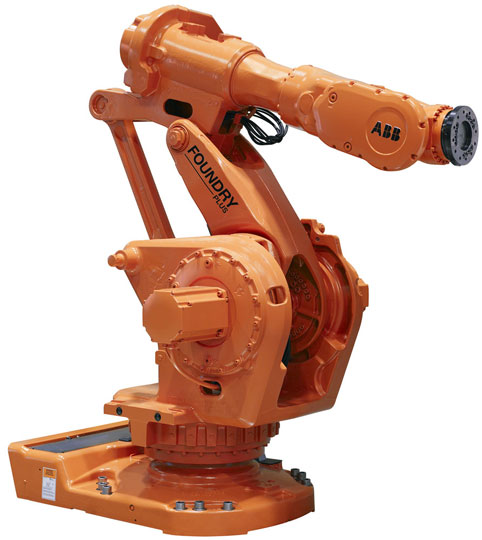
\includegraphics[width=3.5cm, height=4cm]{/serial_abb.jpg}
			\end{center}
		\end{figure}

		\subsection{Configuraciones típicas y parámetros característicos}
			****Según la geometría de su estructura mecánica, un manipulador puede ser:

			\begin{itemize}
				\item{Cartesiano, cuyo posicionamiento en el espacio se lleva a cabo mediante articulaciones lineales.}

				\item{Cilíndrico, con una articulación rotacional sobre una base y articulaciones lineales para el movimiento en altura y en radio.}

				\item{Polar, que cuenta con dos articulaciones rotacionales y una lineal.}

				\item{Esférico (o de brazo articulado), con tres articulaciones rotacionales.}

				\item{Mixto, que posee varios tipos de articulaciones, combinaciones de las anteriores. Es destacable la configuración SCARA (Selective Compliance Assembly Robot Arm).}

				\item{Paralelo, posee brazos con articulaciones prismáticas o rotacionales concurrentes.}
			\end{itemize}

Los principales parámetros que caracterizan a los robots industriales son:

	\begin{itemize}
		\item{Número de grados de libertad. Es el número total de grados de libertad de un robot, dado por la suma de g.d.l. de las articulaciones que lo componen. Aunque la mayoría de las aplicaciones industriales requieren 6 g.d.l., como las de soldadura, mecanizado y almacenamiento, otras más complejas requieren un número mayor, tal es el caso de las labores de montaje.}

		\item{Espacio de accesibilidad o espacio (volumen) de trabajo. Es el conjunto de puntos del espacio accesibles al punto terminal, que depende de la configuración geométrica del manipulador. Un punto del espacio se dice totalmente accesible si el PT puede situarse en él en todas las orientaciones que permita la constitución del manipulador y se dice parcialmente accesible si es accesible por el PT pero no en todas las orientaciones posibles. En la figura inferior se aprecia el volumen de trabajo de robots de distintas configuraciones.}

		\item{Capacidad de posicionamiento del punto terminal. Se concreta en tres magnitudes fundamentales: resolución espacial, precisión y repetibilidad, que miden el grado de exactitud en la realización de los movimientos de un manipulador al realizar una tarea programada.}

		\item{Capacidad de carga. Es el peso que puede transportar el elemento terminal del manipulador. Es una de las características que más se tienen en cuenta en la selección de un robot dependiendo de la tarea a la que se destine.}

		\item{Velocidad. Es la máxima velocidad que alcanzan el PT y las articulaciones.}
	\end{itemize}

		\begin{figure}[htb]
			\begin{center}
			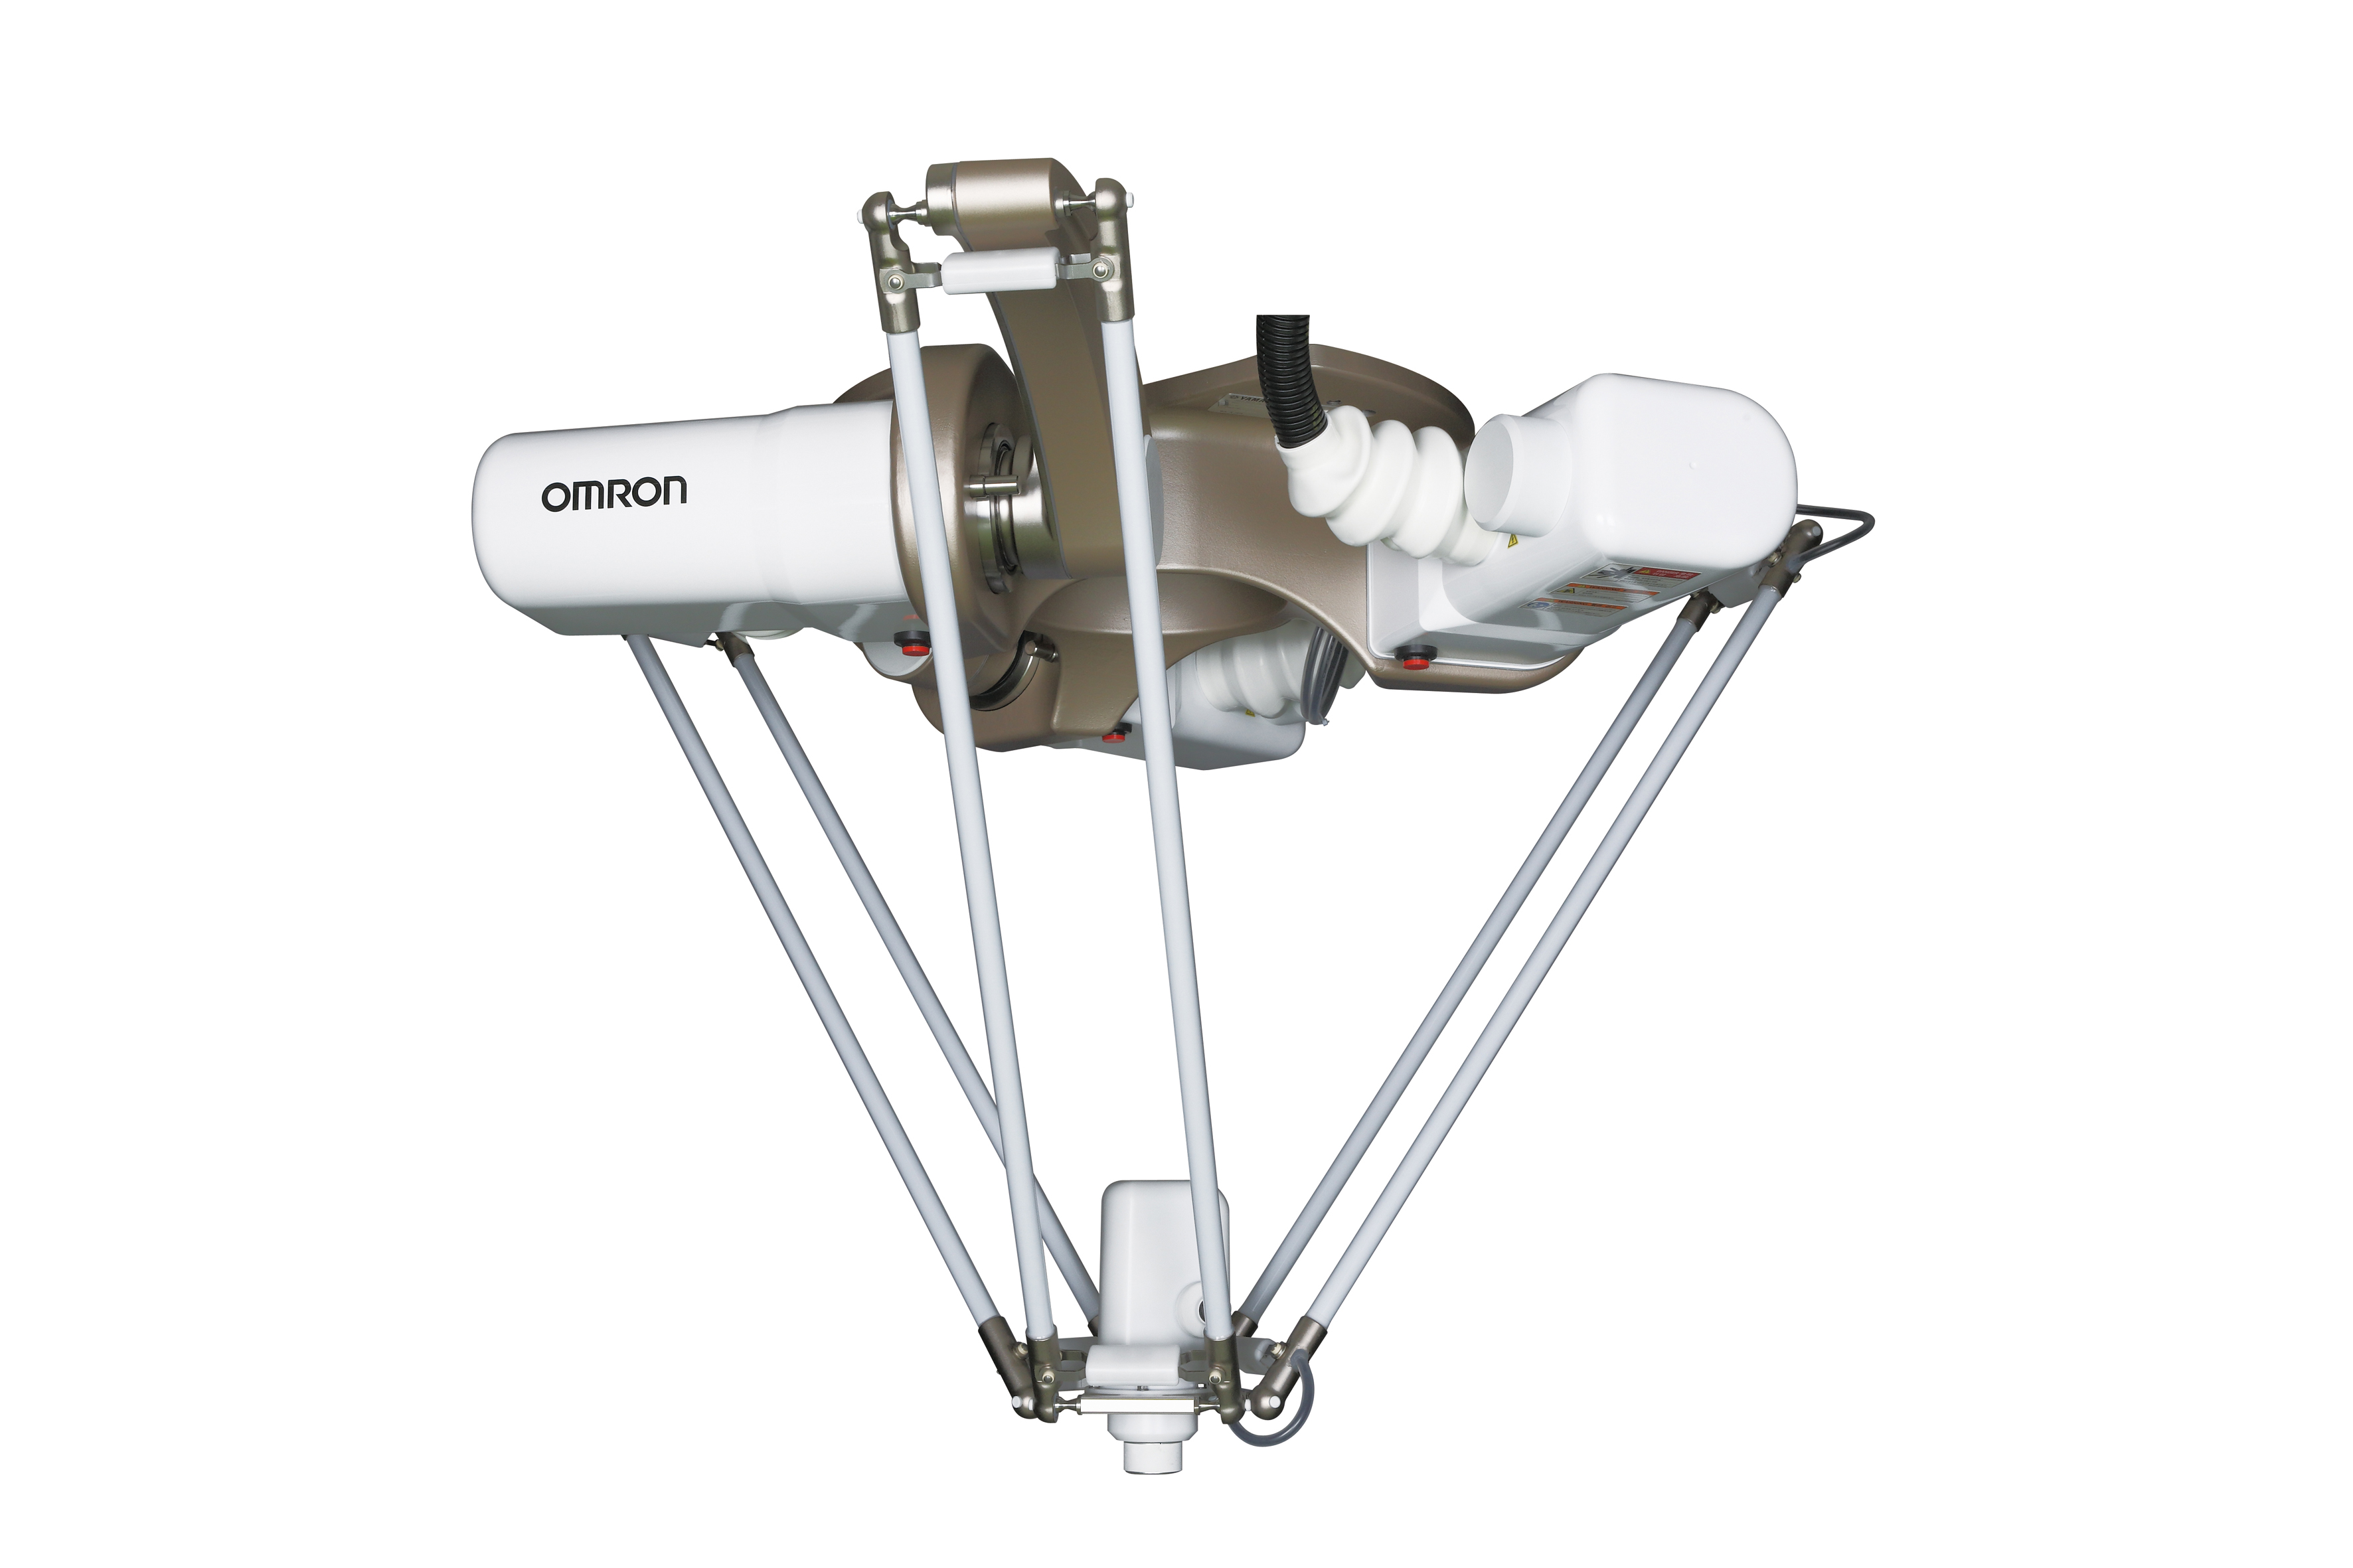
\includegraphics[width=6.5cm, height=4.5cm]{/robotParalelo.jpg}
			\end{center}
		\end{figure}


		\subsection{Descripciones espaciales y transformaciones}
			*La cinemática es la ciencia del movimiento que trata el tema sin considerar las fuerzas que lo ocasionan. Dentro de esta ciencia se estudian la posición, la velocidad y la aceleración. En conseciencia, el estudio de la cinemática de manipuladores se refiere a todas las propiedades geométricas y las basadas en los cambios de estas a lo largo del tiempo. Dadas las características de este trabajo solo se abordarán la cinemática directa e inversa, sin llegar a analizar la dinámica del manipulador.\\

			*El problema de la cinemática directa se plantea en términos de encontrar una matriz de trasformación que relaciona el sistema de coordenadas ligado al cuerpo en movimiento respecto a un sistema de coordenadas que permanece estático y se toma como referencia. Para lograr esta representación se usan la matriz de transformación homogénena con una dimension 4x4, la cual incluye las operaciones de rotación y translación.\\

			*La matriz de transformación homogénea es una matriz de 4x4 que trasnforma un vector expresado en coordenadas homogéneas desde un sistema de coordenadas hasta otro sistema de coordenadas. La matriz de transformación homogénea tiene la siguiente estructura:\\

			***Matriz Transformación Homogénea

			donde los vectores n, s, a, son vectores ortogonales unitarios y p es un vector que describe la posición x, y, z del origen del sistema actual respecto del sistema de referencia.

			*** Gráfico sistemas de referencia.







%%  Imagenes RGD y Points Clouds
%%  ----------------------------------------------
	\section{Imágenes RGB-D}
		En la robótica de servicios resulta imprescindible contar con robots que sean capacez de percibir su entorno, los elementos que los rodean y determinar características de los mismos. Los humanos, dadas estas necesidades, hemos desarrollado el sentido de la vista que nos permite determinar características del entorno y de los objetos que lo componen tales como el color, la forma, las dimensiones o su ubicación en el espacio.\\

		En este sentido la visión artificial es la disciplina encargada de estudiar los procesos de reconocer y localizar objetos en el entorno. Entender estos procesos nos ayudará a construir máquinas con capacidades similares.\\


		\subsection{Características de las imágenes RGB-D}



	\section{Algoritmo RANSAC}
	\section{Algoritmo PCA}
	\section{Características del objeto}


	\section{Planeación de tareas}

